
%%%%%%%%%%%%%%%%%%%%%%% file typeinst.tex %%%%%%%%%%%%%%%%%%%%%%%%%
%
% This is the LaTeX source for the instructions to authors using
% the LaTeX document class 'llncs.cls' for contributions to
% the Lecture Notes in Computer Sciences series.
% http://www.springer.com/lncs       Springer Heidelberg 2006/05/04
%
% It may be used as a template for your own input - copy it
% to a new file with a new name and use it as the basis
% for your article.
%
% NB: the document class 'llncs' has its own and detailed documentation, see
% ftp://ftp.springer.de/data/pubftp/pub/tex/latex/llncs/latex2e/llncsdoc.pdf
%
%%%%%%%%%%%%%%%%%%%%%%%%%%%%%%%%%%%%%%%%%%%%%%%%%%%%%%%%%%%%%%%%%%%


\documentclass[runningheads,a4paper]{llncs}

\usepackage{amssymb}
\setcounter{tocdepth}{3}
\usepackage{graphicx}

\usepackage[outdir=./]{epstopdf}
\usepackage[spanish,es-noshorthands]{babel}
\graphicspath {{images/}}
\usepackage{todonotes}
\usepackage{Tikz}
\usepackage{pspicture}
\usepackage{subfigure}
\usepackage{soul}

\usepackage{url}
%\urldef{\mailsa}\path|{alfred.hofmann, ursula.barth, ingrid.haas, frank.holzwarth,|
%\urldef{\mailsb}\path|anna.kramer, leonie.kunz, christine.reiss, nicole.sator,|
%\urldef{\mailsc}\path|erika.siebert-cole, peter.strasser, lncs}@springer.com|    
%\newcommand{\keywords}[1]{\par\addvspace\baselineskip
%\noindent\keywordname\enspace\ignorespaces#1}

\begin{document}

\title{
	Visualización de Redes Sociales para la Identificación de Bandas Delictivas: Aplicación del Algoritmo de PageRank y Detección de Comunidades
}

\titlerunning{PageRank y Detección de Comunidades en Bandas Delictivas}
\authorrunning{S. Wahler, M. Larrea, D. Martínez}

\author{Sebastián P. WAHLER\inst{1} \inst{2} \and Martín L. LARREA\inst{3} \and Diego C. MARTÍNEZ\inst{3} }
%
% First names are abbreviated in the running head.
% If there are more than two authors, 'et al.' is used.
%
\institute{
	\inst{}Departamento de Informática, Facultad de Ingeniería, Universidad Nacional de la Patagonia San Juan Bosco, Mitre 655, U9100, Trelew, ARGENTINA.\\
	\url{http://www.ing.unp.edu.ar/dpto-informatica.html}
	\and
	\inst{}Departamento de Informática, Procuración General, Ministerio Público Fiscal, Poder Judicial de la Provincia del Chubut, Belgrano 521, U9102, Rawson, ARGENTINA.\\
	\url{https://www.mpfchubut.gov.ar}
	\and
	\inst{}Departamento de Ciencias e Ingeniería de la Computación, Universidad Nacional del Sur, Av. Alem 1253, B8000CPB Bahía Blanca, ARGENTINA.\\
	\url{https://cs.uns.edu.ar/} \\
	\email{(e-mail: spwahler@ing.unp.edu.ar, dcm@cs.uns.edu.ar, mll@cs.uns.edu.ar)}\\	
}
\maketitle              % typeset the header of the contribution

%
\begin{abstract}
	Se presenta el resultado del estudio de las técnicas y metodologías actuales de análisis inteligente de datos y visualización para la asistencia en la investigación criminal, a partir de los registros de actividades delictivas, sus autores y las relaciones de datos que puedan derivarse a partir de ellas. Es de especial interés la identificación de  bandas delictivas o criminales para propender a una persecución penal inteligente. Se discute el desarrollo de un componente de software para la visualización, incorporando la utilización del algoritmo de PageRank y detección de comunidades.  
	\keywords{Investigación Criminal \& Análisis Inteligente de Datos \& Redes Sociales \& Visualización \& PageRank}
\end{abstract}

%
\section{Introducción}

En la actualidad las actividades criminales habituales en una ciudad o región van desde hurtos y robos de poca importancia, hasta otros de mayor gravedad como abusos sexuales y  homicidios. Todos ellos son registrados de diferentes formas por las fuerzas de la ley, con datos de variada precisión que incluyen usualmente la tipificación del delito, los datos en tiempo y espacio, y en muchas ocasiones los autores correspondientes.
Toda esta información respalda los procesos de investigación judicial de cada caso, pero con el transcurso del tiempo constituyen una extensa base de conocimiento sobre la cual es posible extraer valiosa información para la prevención del delito y la búsqueda de la justicia. 
Por ejemplo, es posible inferir relaciones de amistad o conveniencia entre diversos autores de actividades criminales a partir de los registros delictivos y es de extrema relevancia para la prevención del delito y la resolución de casos inconclusos.
Las organizaciones criminales son grupos que operan fuera de la ley, realizando actividades ilegales en beneficio propio y en detrimento de otros individuos o grupos sociales~\cite{finckenauer2005problems}. Pueden ser de diverso tamaño y cubrir áreas geográficas variadas, en muchos casos en conflicto con otras organizaciones similares. Una de las características particulares de este tipo de organizaciones es que, al estar enfocadas en actividades ilegales perseguidas por los organismos de seguridad pública, el anonimato y/o la discreción de sus miembros es de vital importancia. Esto requiere estudios de la información existente con el fin de identificar los criminales y realizar acciones apropiadas para la prevención del delito.
Los miembros de las organizaciones criminales tienen a su vez diversos grados de compromiso con cada una de ellas. En muchos casos los hechos son cometidos por individuos de baja jerarquía y responsabilidad en el grupo. Asimismo, existen otros individuos de mayor jerarquía y responsabilidad en la organización criminal, que ostentan cualidades de liderazgo.
En tal sentido, con el objetivo de ayudar en la identificación de las bandas delictivas, sus integrantes y el grado de importancia de cada uno dentro de ellas, son de interés dos áreas de las Ciencias de la Computación: el área de Visualización de Información, en particular la Visualización de Grandes Conjuntos de Datos, que busca asistir a los usuarios en la adecuada comprensión de la información, y el Análisis de Redes Sociales, en donde se emplean técnicas y formalismos para la comprensión de las estructuras de las redes y sus nodos . 
En particular, la aplicación de técnicas visuales para la representación de este tipo de información no es nueva ~\cite{xu2005criminal}~\cite{feng2019big}~\cite{mathew2021criminal}. También es importante el estudio de las tareas e interacciones que la visualización debe soportar ~\cite{chen2005visualization}, ya que son estas interacciones las que facilitan la exploración de la visualización de información.
En este trabajo es de especial interés la aplicación de estas técnicas y tecnologías, como así también el desarrollo de un módulo de software para  la visualización de los datos, incorporando nociones de análisis de grafos, como la utilización del algoritmo de PageRank y la detección de comunidades, en pos de encontrar delincuentes de relevancia. Para esto se cuenta con los registros de actividades criminales a través de la colaboración del Ministerio Público Fiscal de la provincia del Chubut, como se detalla en la siguiente sección.

Las organizaciones criminales son grupos que operan fuera de la ley, realizando actividades ilegales en beneficio propio y en detrimento de otros individuos o grupos sociales~\cite{finckenauer2005problems}. Pueden ser de diverso tamaño y cubrir áreas geográficas variadas, en muchos casos en conflicto con otras organizaciones similares. Una de las características particulares de este tipo de organizaciones es que, al estar enfocadas en actividades ilegales perseguidas por los organismos de seguridad pública, el anonimato y/o la discreción de sus miembros es de vital importancia. Esto requiere estudios de la información existente con el fin de identificar los criminales y realizar acciones apropiadas para la prevención del delito.

Los miembros de las organizaciones criminales tienen a su vez diversos grados de compromiso con cada una de ellas. En muchos casos los hechos criminales que son evidentes en la sociedad ocurren por individuos de baja jerarquía y responsabilidad en el grupo, motivados por la recompensa inmediata, las aspiraciones de ascenso y la reputación en su propio círculo de contactos. Asimismo, existen otros individuos de mayor jerarquía y responsabilidad en la organización criminal, que ostentan cualidades de liderazgo, intereses a largo plazo, y la constante preocupación por la conservación del poder para el beneficio personal y de la organización. Con frecuencia, son los individuos del primer grupo los que cometen delitos percibidos y registrados por las fuerzas policiales, mientras que los miembros del segundo grupo se mantienen con mayor discreción. Adicionalmente, las estructuras jerárquicas, la forma de operar, y la cultura inherente de sus realidades socio-económicas  imponen códigos propios que hacen difícil la identificación de la organización delictiva como un todo, con sus miembros y actividades relacionadas. Es aquí donde nuestro trabajo puede aportar un rol significativo.

\section{Análisis de Redes Sociales (SNA)}

Desde hace algunos pocos años, el Análisis de Redes Sociales (o SNA por sus siglas en inglés de Social Network Analysis) ha contribuido a las investigaciones criminales y a las actividades de inteligencia relacionadas.
Una red social modela individuos como nodos, vinculados entre sí por arcos o aristas que representan las relaciones entre esos individuos. El estudio de estas redes es importante porque se enfoca en la abstracción de las relaciones humanas sobre uno o más aspectos particulares ~\cite{pm2018practical}~\cite{burcher2020social}. De esta manera, las redes conforman estructuras de grafos en las cuales es posible identificar diversas propiedades, tales como la relevancia o la importancia relativa de los nodos individuales en función de las conexiones existentes o el flujo de información. Según Sage~\cite{scott2011sage} , existen cuatro pilares fundamentales del análisis de redes: el reconocimiento de la importancia de las relaciones sociales entre los individuos, la recolección y análisis de datos sobre estas relaciones, la importancia de la representación visual de estos datos y la necesidad de modelos matemáticos y computacionales que expliquen los patrones de conexión entre los individuos.

En particular, la vinculación entre el estudio de las redes sociales y la investigación criminal ha sido encarada por varios autores. A mediados de los 70 se utilizaban modelos básicos para establecer y cualificar las relaciones entre individuos o actores de un escenario particular, definiendo grafos de acuerdo a la información recolectada~\cite{harper1975application}, pero el procesamiento era mayoritariamente manual y con varias etapas de refinamiento y valoración de datos. Esta es la que según Klerk~\cite{Klerks1999TheNP} sería la primera generación de análisis de redes en criminalística. La segunda generación involucra el uso de herramientas computacionales que automatiza parte de la tarea de registro y estructuración de datos. Estas herramientas además aumentaron notoriamente la cantidad de datos que se pueden analizar, haciendo mucho más ágil su registro y consulta. La tercera y actual generación establece la definición de modelos y técnicas matemáticas para la generación de nuevo conocimiento, como la identificación de posiciones de poder e influencia o la calidad de potenciales testigos o informantes. Métricas como la centralidad de un nodo en un grafo son especialmente útiles en este escenario.

Uno de los trabajos más importantes al respecto es el de Krebs ~\cite{krebs2002mapping}, en donde se identifica una parte de la red de terroristas que fue responsable de los atentados del 11 de septiembre de 2001 en Nueva York. Aquí identifica agrupaciones de individuos que se conectan entre sí por los pilotos responsables del secuestro de las aeronaves. Otros estudios similares han sido efectivos en consecuencia ~\cite{medina2014social}~\cite{qin2005analyzing}~\cite{stollenwerk2016taking}.  Por otro lado, el análisis de redes sociales ha cobrado también interés en la investigación criminal tradicional como las estructuras de la mafia o el narcotráfico ~\cite{bouchard2013advances}~\cite{bright2015use}~\cite{giommoni2017illicit}~\cite{morselli2009hells}~\cite{morselli2010assessing}. Estudios como el de Malm ~\cite{malm2011networks} han permitido identificar roles en la cadena de suministros para la fabricación de drogas ilícitas, lo que acarrea diferentes riesgos penales para cada uno de los colaboradores. Otros estudios se enfocan en el uso del análisis de las redes sociales para otras actividades criminales, como el tráfico ilícito de arte ~\cite{bichler2013small}, el lavado de dinero ~\cite{colladon2017using}~\cite{soudijn2014using}, corrupción policial ~\cite{lauchs2011corrupt} y bandas juveniles ~\cite{mcgloin2005policy}~\cite{bichler2014magnetic}. Existen también líneas de investigación en la disciplina referente al cibercrimen ~\cite{decary2014information}~\cite{decary2012social}~\cite{decary2013reputation}. Es claro entonces que el análisis de redes sociales puede ser aplicado a un amplio rango de actividades criminales y ha demostrado modelar apropiadamente características propias de las organizaciones ilegales, asistiendo a la prevención del delito y al diseño de políticas adecuadas para enfrentar estas actividades.

Existen sin embargo algunas dificultades que requieren aún estudios intensivos. La cantidad de información que debe manejarse es enorme, en muchos casos con información incompleta, contradictoria y no menos frecuentemente incorrecta. Además, las relaciones humanas tradicionales se mezclan naturalmente con las interacciones ilícitas entre los individuos por lo que es necesario identificar apropiadamente su naturaleza y consecuencias y determinar los límites sensatos de la red social analizada. 

Actualmente los organismos estatales encargados de la Justicia y la prevención del delito cuentan con registros informatizados de las actividades criminales detectadas, así como de las etapas y eventos del subsecuente proceso penal. En particular, para este trabajo es de especial interés la información producida a tal efecto por las fuerzas policiales de la Provincia del Chubut y su Poder Judicial de la mano del Ministerio Público Fiscal (MPF). Existen decenas de miles de registros que son utilizados principalmente para la acción penal, pero que pueden ser empleados para modelar diferentes redes sociales sobre las cuales aplicar un análisis matemático y computacional en la búsqueda de nueva información. Esto permitirá conocer más sobre las actividades criminales y sus autores en la jurisdicción de esa provincia, con las particularidades propias de la información registrada digitalmente.

El análisis y exploración de estos grandes conjuntos de datos y sus relaciones debe ser asistido por técnicas y herramientas que faciliten este proceso y reduzcan la carga cognitiva que recae sobre los usuarios. En tal sentido, el área de Visualización de Información, en particular la Visualización de Grandes Conjuntos de Datos, busca asistir a los usuarios de tal manera. La aplicación de técnicas visuales para la representación de este tipo de información no es nueva ~\cite{xu2005criminal}~\cite{feng2019big}~\cite{mathew2021criminal}. También es importante el estudio de las tareas e interacciones que la visualización debe soportar ~\cite{chen2005visualization}, ya que son estas interacciones las que facilitan la exploración de la visualización de información.


\section{Marco de Trabajo - Ministerio Público Fiscal del Chubut}
\vspace{-5pt}
Desde hace pocos años, el Análisis de Redes Sociales (o SNA por sus siglas en inglés de Social Network Analysis) ha contribuído a las investigaciones criminales y a las actividades de inteligencia relacionadas.
Actualmente los organismos estatales encargados de la Justicia y la prevención del delito cuentan con registros informatizados de las actividades criminales detectadas, así como de las etapas y eventos del subsecuente proceso penal. 
Esta información constituye en esencia, una forma de \textit{red social}. 
Para este trabajo es de especial interés la información producida por las fuerzas policiales de la Provincia del Chubut y su Poder Judicial de la mano del Ministerio Público Fiscal (MPF ~\cite{MPFChubutPaginaWeb}), registradas en el sistema \texttt{Coirón}. 
%Este es el sistema informático que colabora con la administración del flujo de casos ingresados al MPF~\cite{MPFChubutPaginaWeb}. 
Ésta es una herramienta que permite registrar, comunicar y gestionar las actividades, trámites y actuaciones que se realizan para un caso penal, desde la denuncia hasta su finalización. También es una herramienta de administración de información, flujo de casos, planificación, organización, coordinación y control.
%Ha sido desarrollado a medida de las necesidades del MPF, adaptado al Código Procesal Penal vigente y a los lineamientos estratégicos definidos. 
Su progreso, mantenimiento y mejora continua está a cargo del Equipo de Desarrollo del Departamento de Informática del Área de Planificación y Control de Gestión de la Procuración General.
Entre otras funcionalidades, es de interés la incorporación de herramientas de visualización de información, potenciando el análisis que realizarán luego los especialistas de análisis criminal.
En este trabajo nos enfocamos en las bandas delictivas y la \textit{importancia relativa} de sus integrantes. 
Para ello es central el concepto de "\textit{Grupo de Pertenencia}", como se denomina en el Sistema \texttt{Coirón} a la relación directa que existe entre un individuo dentro del universo de personas cargadas como actores de delitos (roles: denunciado, sospechoso o imputado) y otros individuos del mismo universo, con los cuales existan uno o más casos penales en común.
El objetivo es contar con componentes de software que 
%Crear un módulo de software "Red de Grupos de Pertenencia" donde se 
muestren gráficamente las relaciones entre las personas involucradas en los casos penales, enriquecida con información proveniente de la analítica de grafos. 
%La idea es no sólo enfocarse en el grupo de pertenencia de una persona en particular, sino que mediante herramientas inteligentes, una visualización apropiada y con diversos filtros de búsqueda, se logre mostrar las relaciones entre un determinado grupo de personas y de esta manera poder inferir la conformación de posibles bandas delictivas.

En estos grafos un nodo es una persona (con los roles ya mencionados) si está involucrada en dos o más casos penales \footnote{Existe un gran cúmulo de personas en el sistema con sólo un caso con rol de \textit{denunciado}, por esa razón se los excluye del universo a analizar. Serían parte del dataset a visualizar si se encuentran relacionados con otros nodos del primer grupo.}. El tamaño del nodo posee una relación directa con la cantidad de casos penales en los que se encuentre involucrada la persona. Cuanto mayor sea el tamaño del nodo, mayor es la cantidad de casos penales en las que está involucrado.
Los arcos entre pares de nodos vinculan a las personas entre sí y representan el o los casos que tienen en común. El grosor de la vinculación será directamente proporcional a la cantidad de casos en común entre un par de personas. Hay nodos que se encontrarán aislados en el grafo, y esto no significa que no estén efectivamente involucrados en casos, sino que quizás no existan relaciones para el filtro de búsqueda que se utilice en esa vista en particular.

Supongamos que una persona $A$ se encuentra asociada a 8 casos penales, una persona $B$ a 4 y una persona $C$ a 2 casos. 
Las personas $A$ y $B$ se encuentran relacionadas entre sí, por estar en 3 casos en común (casos 1, 2 y 3). Por otro lado las personas $A$ y $C$ también se encuentran relacionadas, por tener un caso en común (caso 4).  Una representación gráfica de dicha situación se muestra en la Figura \ref{fig:grafode2}, y puede observarse el doble de tamaño entre el nodo $A$ y el nodo $B$, representando justamente la diferencia de casos entre ambos nodos (8 y 4 casos). También se ve a simple vista el grosor del enlace entre $A$ y $B$ tres veces más grande que el enlace entre $A$ y $C$ (3 casos en común entre el primer par de nodos, y sólo un caso para el último par de nodos mencionado). 


%\vspace{-15pt}
\begin{figure}
	\centering
	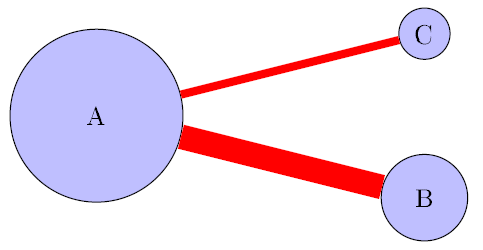
\includegraphics[width=0.25\linewidth]{grafo-ejemplo.png}
	\caption{Ejemplo de relación entre tres personas.} 
	\label{fig:grafode2}
\end{figure}
%\vspace{-5pt}

Esta es, en primera instancia, una caracterización de la importancia de los individuos en la red.
Sin embargo, analíticas mas complejas podrían aplicarse.

\section{Descripción general de los Datos}
En esta sección, describimos nuestro conjunto de datos de casos penales y la red de personas asociada, así como algunas características interesantes que se han de mencionar.

%\subsubsection{Dataset de Delitos}

Nuestro conjunto de datos consta de casos penales, actuaciones (bitácora de eventos del proceso penal), delitos, personas, elementos (denunciados y secuestrados), todos ellos relacionados, registrados entre octubre de 2006 y mayo de 2022 en la Circunscripción Judicial de Trelew - Chubut. 
Este conjunto de datos incluye lugares relativos a personas y a hechos delictivos, fechas, estados procesales de los casos y las personas, como así también los vínculos entre todos los conjuntos mencionados. 
Son 105586 casos penales, 183348 personas involucradas en casos, un universo de 132950 personas en total y 113010 delitos cargados. En relación al conjunto de datos para la visualización, constituyen: 33178 nodos, 16964 enlaces y 60513 relaciones Nodos/Enlaces.

%\subsubsection{Propiedades de la red}

A partir de los datos de los casos penales, pudimos construir la red de Grupos de Pertenencia. En esta red, se eliminan los nodos de aquellas personas cuyos roles no sean referidos a actores delictivos, como ser: denunciantes, víctimas, damnificados, etc. En la Figura \ref{fig:grafocompleto} se muestra una visualización de la red. En la misma se puede observar un grafo compuesto de más de 30000 personas con más Casos Penales registrados en el Sistema de Gestión Coirón (con los siguientes criterios: involucradas en más de un caso con rol de imputado, sospechoso o denunciado; se incluyen personas fallecidas, menores y personas jurídicas). Se visualizan además en la figura todas las relaciones que existen entre esas personas y sus grupos de pertenencia.
\vspace{-10pt}
\begin{figure}
	\centering
	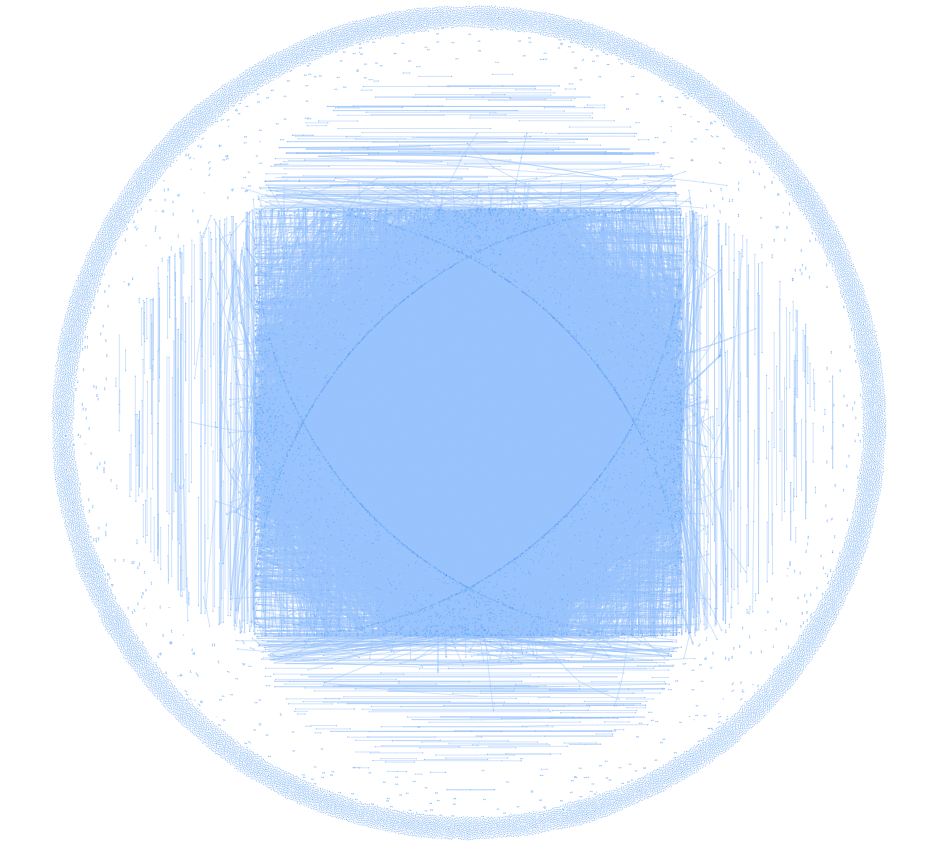
\includegraphics[width=0.4\linewidth]{grafo-30000-completo.png}
	\caption{Más de 30000 personas con más casos y sus relaciones.} 
	\label{fig:grafocompleto}
\end{figure}
\vspace{-10pt}
A los sentidos prácticos de la investigación penal, una visualización con tantos nodos y relaciones no es representativa ni conduce a ningún tipo de detección de bandas delictivas, pero es un claro ejemplo del universo de datos que se disponen en el dataset utilizado, como así también la potencia de la herramienta de visualización. En la Figura \ref{fig:grafosCompletos} se pueden observar ejemplos en los que se han tomado en cuenta los grupos de pertenencia de cada nodo a mostrar, es decir que se visualizan las personas con sus grupos de pertenencias particulares (según parámetros de búsqueda seleccionados). En la imagen (a) se muestran 10000 personas, en (b) 1000 y en (c) 100 personas con más casos y sus grupos de pertenencia relacionados.
\vspace{-10pt}
\begin{figure}[htbp]
	\centering
	\subfigure[Top 10000.]{
		\begin{minipage}[t]{0.33\linewidth}
			\centering
			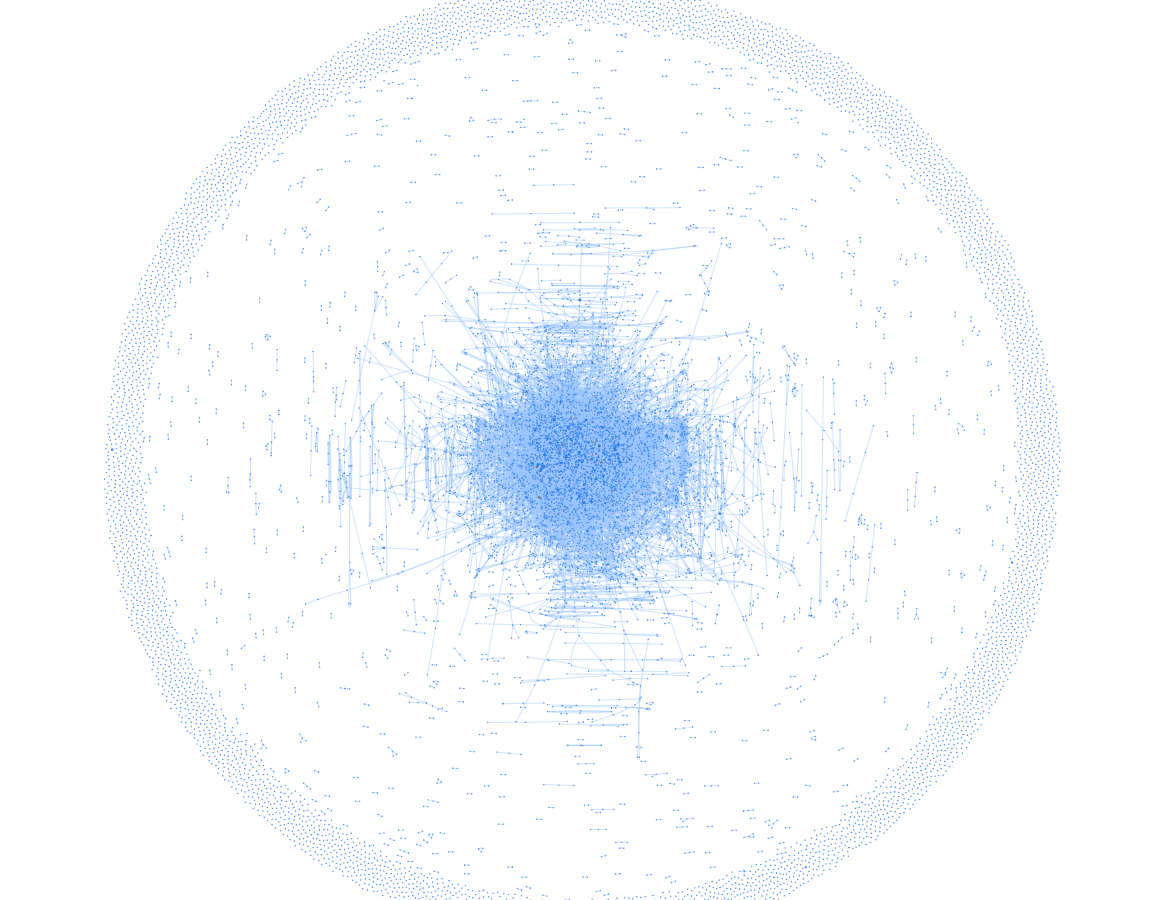
\includegraphics[width=1in]{grafo-10000-completo.png}
			%\caption{fig1}
		\end{minipage}%
	}%
	\subfigure[Top 1000.]{
		\begin{minipage}[t]{0.33\linewidth}
			\centering
			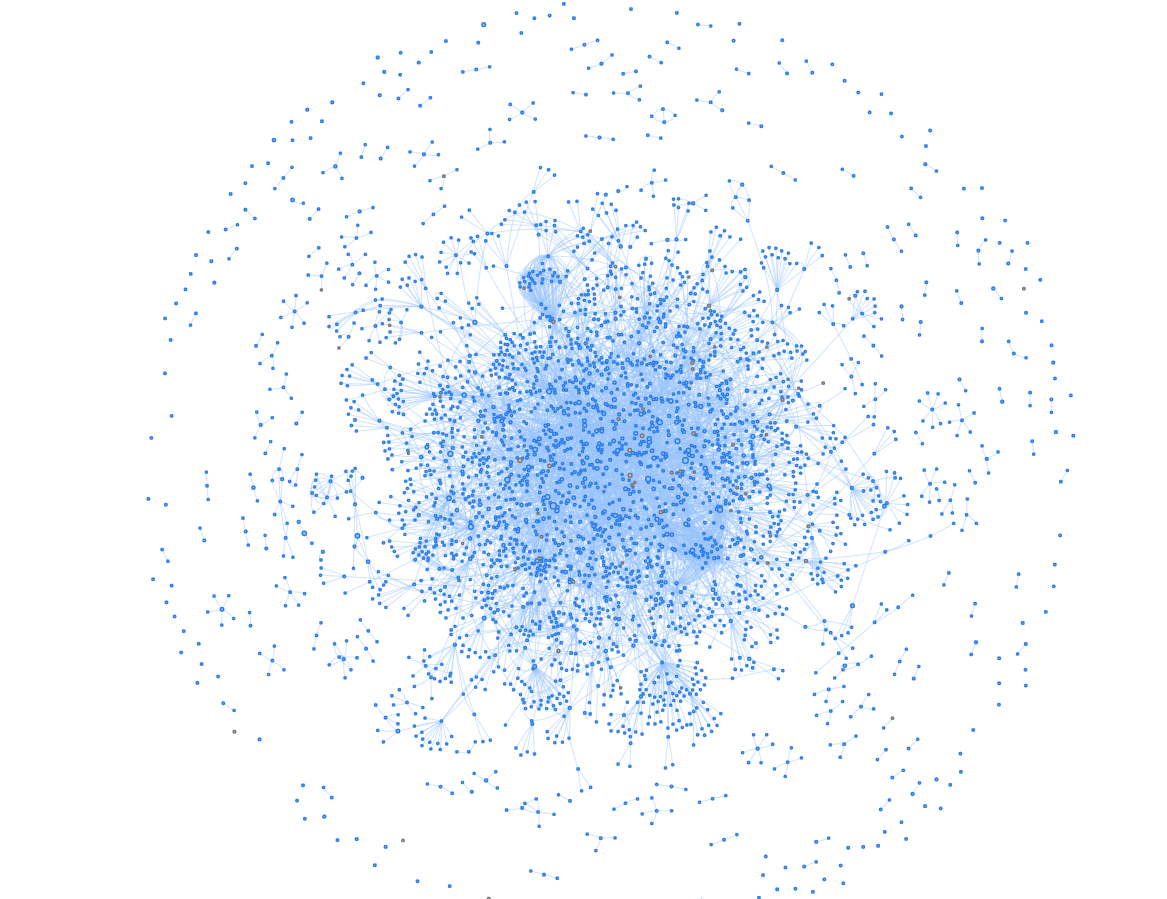
\includegraphics[width=1in]{grafo-1000-completo.png}
			%\caption{fig2}
		\end{minipage}%
	}%
	\subfigure[Top 100.]{
		\begin{minipage}[t]{0.33\linewidth}
			\centering
			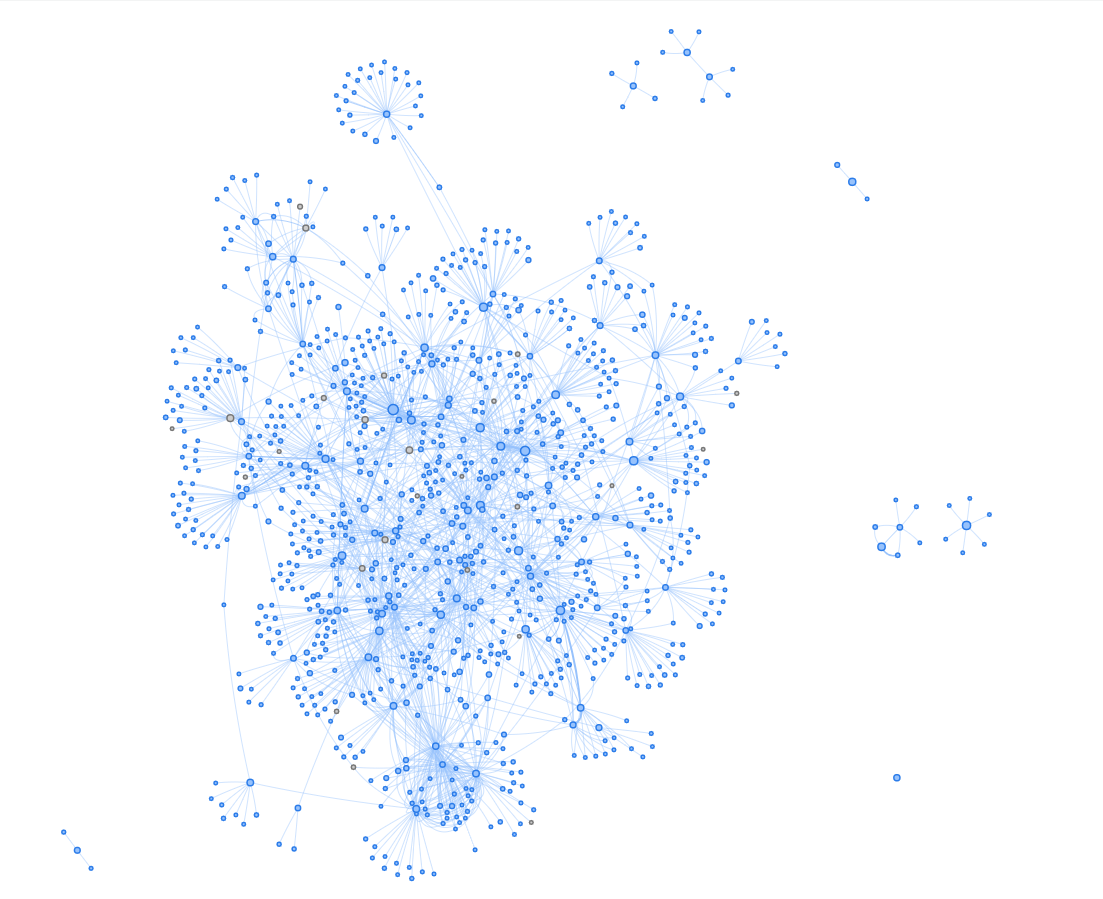
\includegraphics[width=1in]{grafo-100-completo.png}
			%\caption{fig3}
		\end{minipage}
	}%
	\centering
	\caption{ Personas en más casos, con la inclusión de sus grupos de pertenencia particulares.}
	\label{fig:grafosCompletos}
\end{figure}
\vspace{-10pt}
Al analizar la composición de la red obtenida podemos observar las relaciones que existen entre los nodos y como se "equilibra" el grafo, haciendo que aquellos nodos con pocas o nulas relaciones queden en la periferia de la gráfica. Sumado a ello también es apreciable la medida de centralidad de aquellos nodos que son rodeados por sus relacionados. Una aproximación más clara para denotar la medida de centralidad puede verse reflejada en la Figura \ref{fig:grafoTop10}, en donde se visualiza sólo las 10 personas con más Casos y sus grupos de pertenencia. Claramente esos 10 nodos principales quedan rodeados de sus grupos de pertenencia y se pueden observar transitividades entre ellos a través de nodos que conforman parte del grupo de pertenencia de más de un nodo principal.
\vspace{-10pt}
\begin{figure}
	\centering
	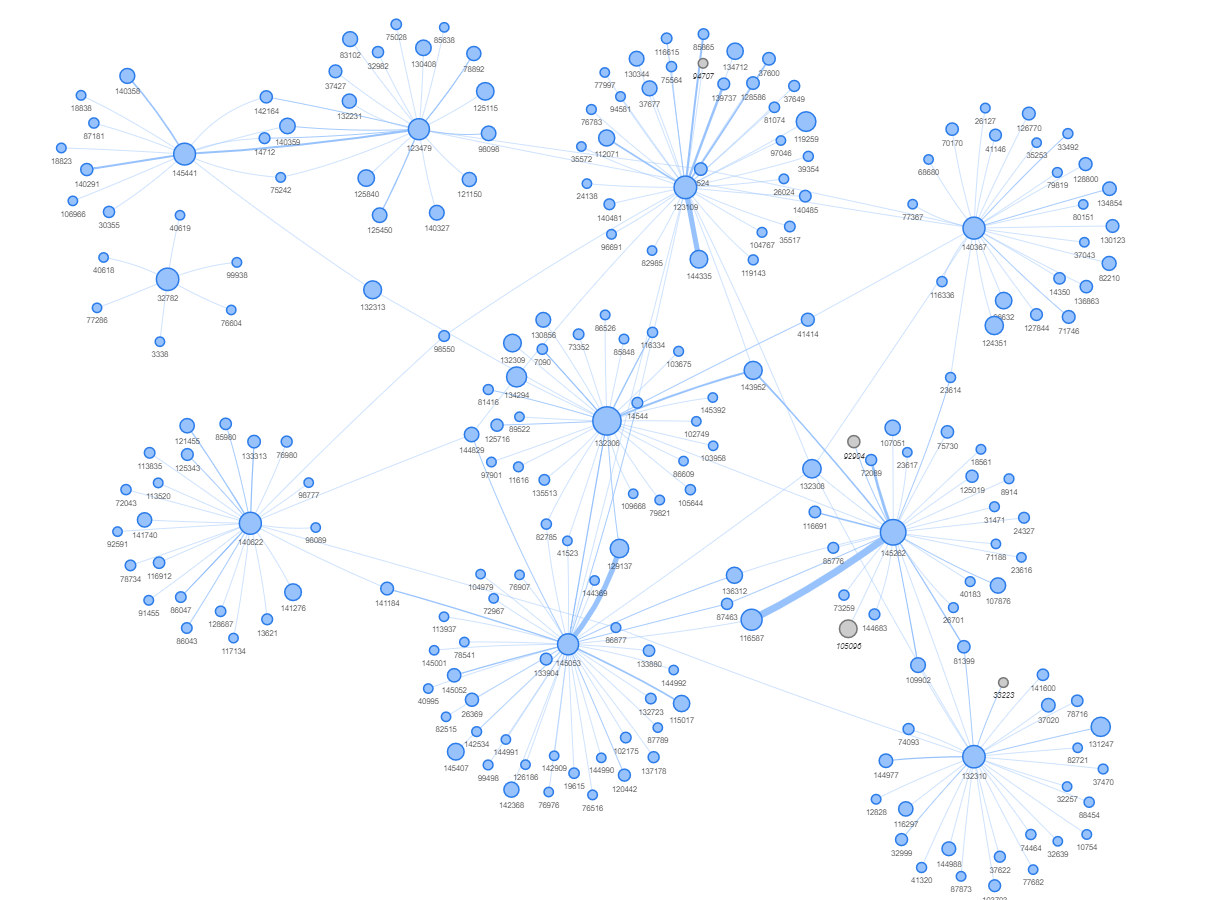
\includegraphics[width=0.5\linewidth]{grafo-10-completo.png}
	\caption{10 personas con más casos en Coirón, con sus relaciones} 
	\label{fig:grafoTop10}
\end{figure}
\vspace{-20pt}
\subsubsection{Centralidad de Grado} La centralidad de grado es una de las medidas más simples de centralidad. En esta se mide el número de enlaces o conexiones que tiene un nodo con los demás nodos pertenecientes a un grafo. Cuando se aplica un análisis de este tipo pueden determinarse diferentes medidas. Por ejemplo, en redes sociales podemos medir el grado de entrada de un nodo como la popularidad o preferencia que posea y la salida definirla como un indicador de sociabilidad. En nuestro caso de estudio, los miembros de las bandas delictivas modifican dinámicamente sus relaciones con otros miembros de la red, lo que resulta en un cambio de su rol e importancia. Una serie de medidas de centralidad de grado pueden ayudar a identificar estos cambios. Estas estadísticas se pueden utilizar para filtrar la vista de la red en función del valor de un nodo específico y resaltar su posición dentro de la red. El grado de centralidad en nuestro grafo se definirá entonces como el número de enlaces directos que tiene un delincuente. Un nodo con un alto grado puede verse como un "centro", un nodo activo e importante en la red~\cite{carley2006destabilization}.
\vspace{-10pt}
\subsubsection{Transitividad} El coeficiente de agrupamiento (transitividad) de un gráfico mide el grado de conexión de una red. Altos coeficientes de agrupamiento significan la presencia de un alto número de triángulos en la red. Es bien conocido en la bibliografía~\cite{wasserman1994social} que las redes sociales muestran valores altos del coeficiente de agrupamiento cuando reflejan la estructura social subyacente de los contactos entre amigos/conocidos. Además, los valores altos del coeficiente de agrupamiento local se consideran un indicador confiable de los nodos cuyos vecinos están muy bien conectados y entre los cuales puede fluir una cantidad sustancial de información.

%\subsubsection{Desarrollo de la Visualización}

Para llevar a cabo la visualización del conjunto de datos obtenidos del análisis inteligente anteriormente descripto, se utilizó Vis.js ~\cite{visjsPaginaWeb}, una biblioteca o librería de visualización dinámica basada en lenguaje Javascript. La misma está diseñada para que sea fácil de usar, para manejar grandes cantidades de datos dinámicos y para permitir la manipulación y la interacción con los datos. La biblioteca consta de los componentes DataSet, Timeline, Network, Graph2d y Graph3d.

En nuestro caso particular utilizamos el componente "Network", que permite mostrar redes en grafos. La visualización es fácil de usar y admite formas, estilos, colores, tamaños, imágenes, etc. Funciona sin problemas en cualquier navegador moderno para hasta unos pocos miles de nodos y bordes. Para manejar una mayor cantidad de nodos, Network tiene soporte de agrupamiento. La red utiliza canvas HTML para la renderización.

Vis.js proporciona implementaciones de algoritmos de diseño forzados "Force-directed graph drawing". Estos algoritmos dirigidos por fuerza intentan posicionar los nodos considerando las fuerzas entre dos nodos (atractivos si están conectados, repulsivos de lo contrario). Generalmente son iterativos y mueven los nodos uno por uno hasta que ya no es posible mejorar o se alcanza el número máximo de iteraciones. Los enlaces tienen más o menos la misma longitud y el menor número posible de enlaces cruzados. Los nodos conectados se juntan más mientras que los nodos aislados se alejan hacia los lados.



\section{Identificación de posibles Bandas Delictivas}
En esta sección, describimos nuestro problema, algunos de los enfoques prácticos existentes utilizados por las fuerzas de la ley y nuestro enfoque basado en la teoría de grafos con características generadas principalmente por la distribución de los datos anteriormente descrita.

\subsubsection{Métodos existentes}
Las personas nos movemos habitualmente entre lugares conocidos o nodos (hogar, trabajo, supermercado, restaurante) y por las mismas calles o rutas. La teoría sugiere que cuando ocurre un delito es porque se cruzan delincuentes y víctimas dentro de algunas de estas zonas de actividad.
Por otro lado se puede deducir que los delincuentes se comportan igual que el resto de las personas. Es decir, un delincuente tenderá a cometer un delito en algún lugar que se encuentre dentro o cerca del recorrido que realiza diariamente para trasladarse.
De ambos enfoques se busca encontrar la mayor cantidad de patrones de ocurrencia entre diversos hechos de similar criminalidad y patrones horarios, como así también las zonas geográficas en donde se producen.  
La naturaleza de los vínculos de los integrantes de una banda delictiva es una variable que aporta información sobre las características y similitudes de los miembros del grupo, atendiendo a criterios concretos: vínculo familiar, cultural, de proximidad (provienen del mismo barrio), han compartido prisión, de especialización (habilidades delictivas), la experiencia u otras capacidades, y otros tipos de vínculo.


\subsubsection{Enfoque propio}
Ante los enfoques teóricos y prácticos estudiados anteriormente, nuestro desarrollo de software propio, que permite mostrar de manera gráfica las relaciones entre actores delictuales en el Sistema Penal de la Provincia del Chubut, se potencia como una herramienta vital de apoyo en la toma de decisiones de la investigación penal de bandas delictivas.

Poder visualizar relaciones entre las personas involucradas en casos penales ayuda a los especialistas a detectar triangulaciones, transitividades y por supuesto centralidades en la Red. Todo ello, sumado a los indicios de investigación y la propia expertís en la temática completan una herramienta de análisis para determinar ciertas bandas o grupos altamente relacionados.

En el año 2019 existieron investigaciones vinculadas a reiterados robos de televisores LCD en domicilios, como así también una serie de hechos consecutivos vinculados al robo de cajas fuertes en empresas del parque industrial de la ciudad de Trelew.

La UAC (Unidad de Análisis Criminal), organismo auxiliar de la Procuración General perteneciente al Ministerio Público Fiscal del Chubut, sirvió como equipo de apoyo en la investigación de ambos modus operandi, haciendo uso de toda la información de los legajos fiscales, consultas generales y específicas contenidas en el Sistema Coirón. Fue de vital uso la información referida a los grupos de pertenencia de cada persona, pero devino en un arduo trabajo entrecruzando información de personas, para dar con las supuestas bandas delictivas detrás de estos hechos.

Dichas investigaciones sirvieron como puntapié inicial para realizar este trabajo y poder facilitar la información ya contenida en el sistema de gestión penal, de otra manera, de una forma más directa y visual a la hora de investigar, que sirva directamente como apoyo a la toma de decisiones en las investigaciones de bandas delictivas. 

A continuación se puede observar una visualización extraída de este trabajo, utilizando como filtros de búsqueda dos personas (nodos 116587 y 145262) con muchos casos y relaciones en el sistema, a fin de encontrar si existe algún tipo de relación directa entre ambos, y a su vez si existen nodos que produzcan transitividades o sean a su vez centrales de otros grupos.
Desde la visualización se agregó gracias a la vinculación con el sistema de la oficina de identificación de personas, fotografías para colocar en los nodos y hacer de este trabajo una herramienta aún más potente. Aquellas personas que no hayan sido identificadas en sede judicial no tendrán fotografía. Por cuestiones judiciales se han desenfocado las fotografías y se han colocado identificadores en vez de los nombres reales de las personas intervinientes.
\vspace{-10pt}
\begin{figure}
	\centering
	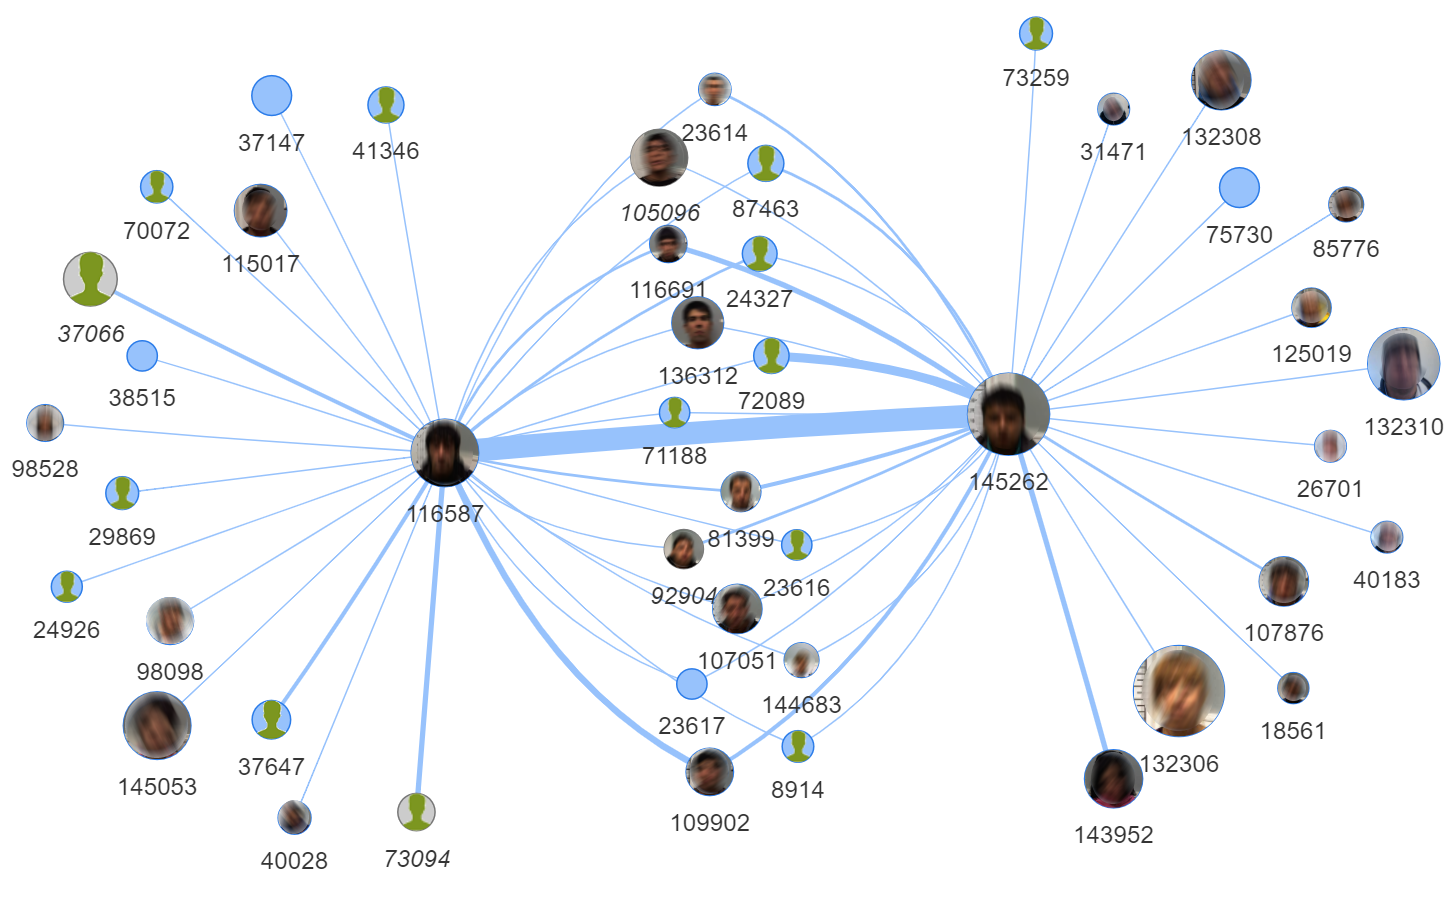
\includegraphics[width=0.75\linewidth]{hermanos-curruman.png}
	\caption{Relación entre dos personas. Se agregan fotografías.} 
	\label{fig:hermanos-curruman}
\end{figure}
\vspace{-10pt}
Como puede verse, existen en la parte central de la imagen muchas personas que se encuentran relacionadas delictualmente con ambos nodos en cuestión. De esta manera se pueden tomar acciones con respecto a estas personas en pos de encontrar patrones de ocurrencia que los vinculen ante la posibilidad de identificarlos como una supuesta banda delictiva. 


\section{PageRank y detecciones comunitarias}
Como parte simplificada de la estructura de una comunidad de nodos en una red social, cada uno representa a un individuo y la red tiene una segmentación multitudinaria~\cite{ma2014exploring}. Algunas personas son centrales en la comunidad, algunas están al margen, establecen menos relaciones con otros y, por lo tanto, tienen una influencia menor. En esta sección, presentamos un nuevo enfoque de descubrimiento comunitario basado en el algoritmo PageRank para encontrar a estos delincuentes "importantes" ó con "mayor influencia" en nuestro grafo, con el fin de analizar supuestas bandas delictivas.

Un grafo es un par $G = (N, A, g)$ donde $N$ es un conjunto finito no vacío de elementos denominados \textit{nodos} (vértices), $A$ es un conjunto de arcos y $g$ es una función que asocia a cada arco $a$ perteneciente a $A$ con un par no ordenado $(x, y)$, siendo $x$ e $y$ nodos pertenecientes a $N$. Se dice que $a$ es un arco con vértices extremos $x$ e $y$~\cite{dubinsky1984mathematical}.
\vspace{-10pt}
\subsubsection{PageRank}
(PR) es un método que fue implementado a través de un algoritmo
originalmente utilizado por Google que asigna a cada página web de un conjunto dado, un puntaje que refleja su importancia dentro del conjunto. A este puntaje se lo denomina \textit{valor de PageRank}. Ante una consulta, el buscador utiliza estos puntajes para determinar el nivel de relevancia de las páginas, y retorna en primer lugar aquellas con un puntaje más alto. Para calcular los puntajes, PageRank utiliza la estructura de enlaces de la web~\cite{brin1998anatomy}. Una página web tiene un valor de PageRank alto si es apuntada por muchas otras páginas, o bien si es apuntada por páginas con puntajes altos~\cite{page1999pagerank}. PageRank tiene una base intuitiva en el concepto de \textit{random walks} sobre grafos~\cite{gobel1974random}: supongamos que un navegante aleatorio empieza a navegar la web desde una página cualquiera. El navegante puede hacer clic en forma aleatoria sobre alguno de los enlaces presentes en la página en la que se encuentra actualmente con una probabilidad $d$ a la que se denomina \textit{damping factor}, o bien con probabilidad $1-d$ accede aleatoriamente a cualquier otra página web. Este proceso se repite indefinidamente. Luego, el valor de PageRank de una página $P$ puede ser interpretado como la probabilidad de que el navegante aleatorio se encuentre en $P$ al finalizar el proceso. PageRank es definido formalmente de la siguiente manera ~\cite{franceschet2011pagerank}. Sean $q_i$ el número de enlaces salientes que posee la página $i$ , $n$ el número total de páginas web, $d$ el \textit{damping factor} que por lo general adquiere el valor 0.85, $\pi$ un vector columna denominado \textit{vector PageRank}, y $H = (h_{ij})$ una matriz cuadrada de tamaño $n$ tal que $h_{ij} = 1/q_i$ si existe un enlace desde la página $i$ a la página $j$ , y $h_{ij} = 0$ en caso contrario. El valor $h_{ij}$ corresponde a la probabilidad de acceder a la página $j$ desde la página $i$ en un paso, a partir de hacer clic en alguno de los enlaces que aparecen en esta última. El valor de PageRank correspondiente a la página $j$ es $\pi_j$, y se define recursivamente como se muestra en la ecuación \ref{eqn:ecuacionPageRank}~\cite{lin2010data}.

\begin{equation} 
	\label{eqn:ecuacionPageRank} 
	\pi_j = \frac{1-d}{n} + d \sum_{i=1}^{n} \pi_i h_{ij} 
\end{equation}
\vspace{-20pt}
\subsubsection{Aplicación de PageRank para bandas delictivas}
Nuestro dataset descrito anteriormente se obtiene a partir de consultas SQL a la Base de Datos de Coirón. Para hacer uso del algoritmo de PageRank se decidió incorporarlo dentro de esas consultas SQL de modo de obtener un resultado que pueda ser utilizado para la visualización. Dentro de la consulta original se generaba una tabla para los nodos y otra tabla para las relaciones, de esta manera el software realizado para la visualización obtiene dichos datasets y renderiza el grafo.
Para incorporar el cálculo de PageRank, inicialmente se adecuaron ambas tablas para la utilización de la fórmula, y se necesitó de ciertas tablas temporales para el cálculo. Por un lado se computó el grado de salida de cada nodo \textit{(Out Degree)}, es decir el número de enlaces que lo conectan con otros nodos.
Luego se declara el \textit{damping factor}, en nuestro caso $0.85$, el conteo total de nodos, y se calcula el \textit{PageRank inicial} de cada nodo, para después comenzar la iteración buscando cumplir con la sumatoria de la fórmula.

\begin{multicols}{2}
\tiny{
\begin{verbatim}
INSERT INTO #OutDegree
SELECT #Node.id, COUNT(#Edge.src)
FROM #Node 
LEFT OUTER JOIN #Edge ON #Node.id = #Edge.src
GROUP BY #Node.id
DECLARE @dampingFactor float = 0.85
DECLARE @Node_Num int
SELECT @Node_Num = COUNT(*) FROM #Node
INSERT INTO #PageRank
	SELECT #Node.id, rank = ((1 - @dampingFactor) / @Node_Num)
	FROM #Node 
		INNER JOIN #OutDegree ON #Node.id = #OutDegree.id
DECLARE @Iteration int = 0
WHILE @Iteration < 50
BEGIN
	--Iteration Style
	SET @Iteration = @Iteration + 1
	INSERT INTO #TmpRank
		SELECT #Edge.dst, rank = ((1 - @dampingFactor) / @Node_Num) 
		+ (@dampingFactor * SUM(#PageRank.rank / #OutDegree.degree))
		FROM #PageRank 
			INNER JOIN #Edge ON #PageRank.id = #Edge.src
			INNER JOIN #OutDegree ON #PageRank.id = #OutDegree.id
		GROUP BY #Edge.dst
END
\end{verbatim}
}
\end{multicols}

Una vez finalizado el desarrollo de la fórmula, se procedió a realizar pruebas que corroboren el buen funcionamiento del código. Se realizaron ejemplos para pocos nodos con pocas relaciones, de manera tal que sea sencilla la verificación. Se muestran a continuación el Cuadro \ref{tab:TablaPageRank6Nodos} con los resultados de PageRank para 6 nodos, y la Figura \ref{fig:6nodos-pageRank-sinColor} que refleja la visualización de la misma ejecución. En cada nodo se muestra su posición de PageRank, y entre paréntesis el identificador de cada nodo. Como se puede observar el nodo central por el PageRank calculado es el referido al ID \textit{145053}, cuyas relaciones con 3 nodos pesan sobre las relaciones que poseen el resto de los nodos visualizados en el grafo.
%\vspace{-10pt}
\begin{table}
\centering
\resizebox{120pt}{!}{
\label{tab:TablaPageRank6Nodos}
\begin{tabular}{|l|r|}
	\hline
	\textbf{IdNodo} &  \textbf{PageRank} \\
	\hline
	145053 &  0,286845042094944 \\
	\hline
	145262 &  0,199512347112651 \\
	\hline
	116587 &  0,1910604814502 \\
	\hline
	132310 &  0,109790233522352 \\
	\hline
	123109 &  0,106270247927848 \\
	\hline
	129137 &  0,106270247927848 \\
	\hline
\end{tabular}
}
\vspace{10pt}
\caption{Valores de PageRank por nodo luego de la ejecución del algoritmo}
\end{table}
%\vspace{-20pt}
\begin{figure}
	\centering
	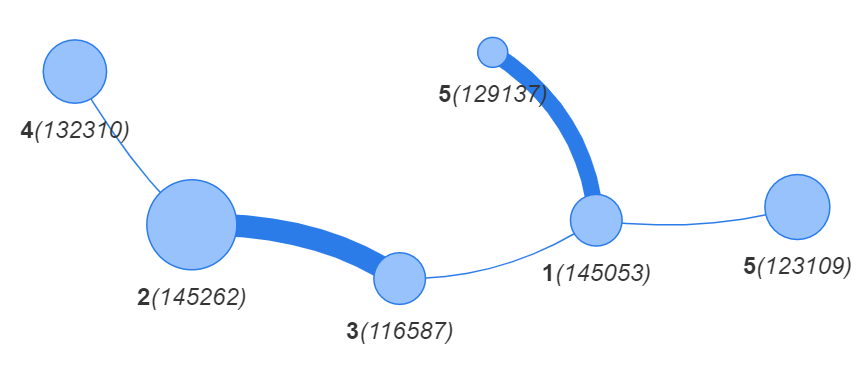
\includegraphics[width=0.50\linewidth]{6nodos-pageRank-sinColor.png}
	\caption{Resultado de ejecución de PageRank para 6 nodos.} 
	\label{fig:6nodos-pageRank-sinColor}
\end{figure}
%\vspace{-30pt}
\vspace{-15pt}
\subsubsection{Detección de comunidades}
Una comunidad puede ser definida como un conjunto de nodos que están más densamente conectados entre ellos que con el resto de la red. La importancia de este planteamiento radica en que se espera que los nodos que están contenidos dentro de una misma comunidad compartan atributos, características comunes o relaciones funcionales  ~\cite{ma2014exploring}.
En este trabajo se aprovecha el algoritmo SQL descrito con anterioridad en el cual se dividen nodos y relaciones para ser luego visualizadas por la herramienta \texttt{Vis.JS}.
En este sentido, nuestro enfoque se basa en la búsqueda de posibles personas que participen en bandas delictivas. Del origen de datos surge que para cada nodo pueden conocerse todas sus relaciones, de modo que podemos asignar a cada uno de esos nodos referentes un identificador de grupo ó cluster. 
Es posible entonces verificar para par de nodos, si pertenecen a un grupo en particular (uno de ellos será "referente" y podremos identificarlo), y de esta manera asignar a cada relación también un grupo determinado. Con ambas tablas (nodos y relaciones) actualizadas, es posible desde la herramienta de visualización, asignar colores a cada cluster, y así generar un grafo aún más práctico a la vista.

Si bien para la visualización se utiliza lenguaje JavaScript de la mano de la librería anteriormente mencionada \texttt{Vis.JS}, y los dataset se obtienen desde la Base de Datos del Sistema \texttt{Coirón} a través de consultas SQL, el software de estudio que toma los datos del dataset y los procesa para luego llamar a la librería de visualización, se encuentra desarrollado en lenguaje C Sharp de .Net Framework. 
A continuación se exhibe en la Figura \ref{fig:grafo-10-completo-ConColor} la misma visualización que se ha presentado con anterioridad en la Figura \ref{fig:grafoTop10}, pero ahora con la detección de grupos por color. Se puede observar que cada grupo o cluster de nodos comparte el mismo color para los enlaces internos. 
\vspace{-10pt}
\begin{figure}
	\centering
	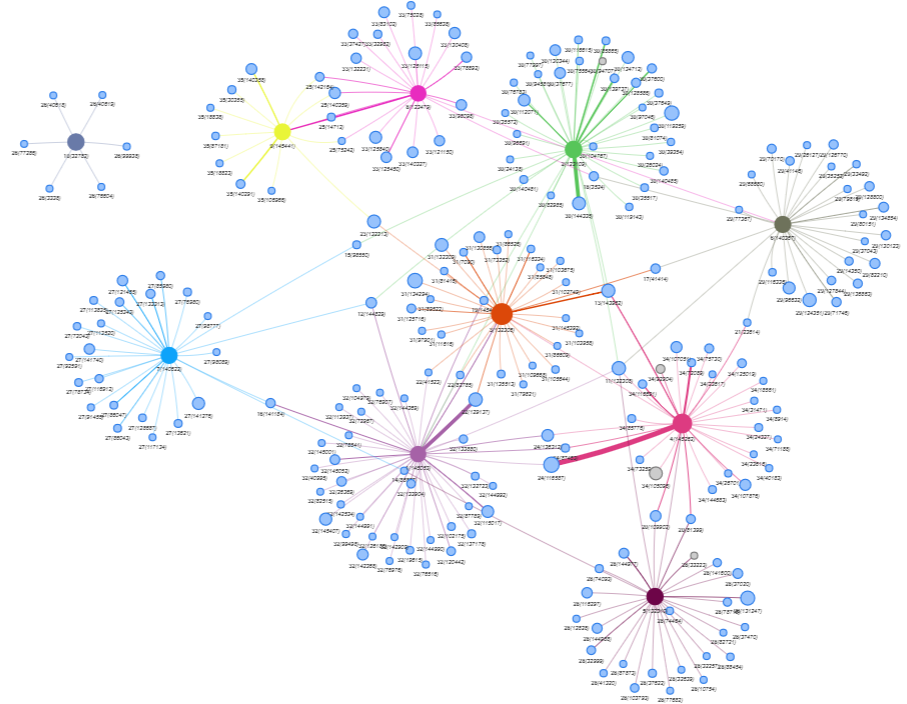
\includegraphics[width=0.5\linewidth]{grafo-10-completo-ConColor.png}
	\caption{10 personas con más casos en Coirón, con sus relaciones. Se agrega detección de comunidades por color.} 
	\label{fig:grafo-10-completo-ConColor}
\end{figure}
\vspace{-30pt}


\section{Conclusiones y trabajos futuros}
En el presente trabajo se propuso un estudio de las técnicas y metodologías actuales de análisis inteligente de datos y visualización para la asistencia en la investigación criminal. Todo ello a partir de los registros de actividades delictivas, sus autores y las relaciones de datos que pueden derivarse a partir de ellas. Fue de especial interés la identificación de redes ilegales, tales como bandas delictivas o criminales para propender a una persecución penal inteligente.

Del estudio propuesto, como se explicó en los capítulos anteriores, se desarrolló un módulo de software como herramienta gráfica para visualizar la red de grupos de pertenencia de los actores delictuales.
El desarrollo de software se implementó en el mismo Ministerio Público Fiscal, del cual se tomaron los datos para generar los datasets de pruebas. De esta manera se ha logrado no sólo estudiar las técnicas y metodologías expuestas, sino también alcanzar la puesta en producción y uso de la herramienta, por los propios actores de la investigación.

Las primeras impresiones de aquellos especialistas de investigaciones penales han sido muy satisfactorias y permiten evaluar a este trabajo como el inicio de futuros desarrollos visuales para el apoyo a la toma de decisiones en la investigación penal.

Como continuación de este trabajo, existen diversas líneas de investigación que quedan abiertas y en las que es posible continuar trabajando; algunas de ellas, están más directamente relacionadas con este trabajo y son el resultado de cuestiones que han ido surgiendo durante la realización del mismo.

Actualmente se 	continúa trabajando en el desarrollo de la aplicación de visualización. Se pretende incorporar a la fórmula original de PageRank, enriquecido con información adicional según los registros judiciales. Por ejemplo, la posibilidad de darle mayor ranking inicial a aquellos nodos que tengan un peso mayor que otros según los registros. También sería interesante hacer lo mismo con el peso que poseen los enlaces entre nodos, ya que no es lo mismo una relación de 2 casos penales en común entre dos personas, que una de 18 casos en común. De esta manera lograríamos darle más ranking también a aquellos nodos que estén relacionados con otros, en mayor cantidad de casos penales. Esto es sin duda relevante para la investigación criminal basada en antecedentes penales.
También se buscará profundizar sobre diversos algoritmos de centralidad. Existen algunas nociones que son de relevancia para la identificación de la importancia de una persona en la red inducida por las causas penales. Por ejemplo, \textit{betweenness centrality}, que modela la medida en que un nodo en particular se encuentra entre otros nodos en una red, o \textit{closeness centrality}, que es la inversa de la suma de los caminos más cortos (geodésicas) que conectan un nodo particular con todos los demás nodos de una red~\cite{newman2005measure}. De manera similar, \textit{eigenvector centrality}, es otra forma de asignar la centralidad a un actor de la red basado en la idea de que si un nodo tiene muchos vecinos centrales, también debería ser central.
 

%\renewcommand{\refname}{Referencias Bibliográficas}
\bibliographystyle{splncs04}
\bibliography{bibliografia}


\end{document}
